\documentclass[de]{agse-empir-report}\usepackage[]{graphicx}\usepackage[]{color}
%% maxwidth is the original width if it is less than linewidth
%% otherwise use linewidth (to make sure the graphics do not exceed the margin)
\makeatletter
\def\maxwidth{ %
  \ifdim\Gin@nat@width>\linewidth
    \linewidth
  \else
    \Gin@nat@width
  \fi
}
\makeatother

\definecolor{fgcolor}{rgb}{0.345, 0.345, 0.345}
\newcommand{\hlnum}[1]{\textcolor[rgb]{0.686,0.059,0.569}{#1}}%
\newcommand{\hlstr}[1]{\textcolor[rgb]{0.192,0.494,0.8}{#1}}%
\newcommand{\hlcom}[1]{\textcolor[rgb]{0.678,0.584,0.686}{\textit{#1}}}%
\newcommand{\hlopt}[1]{\textcolor[rgb]{0,0,0}{#1}}%
\newcommand{\hlstd}[1]{\textcolor[rgb]{0.345,0.345,0.345}{#1}}%
\newcommand{\hlkwa}[1]{\textcolor[rgb]{0.161,0.373,0.58}{\textbf{#1}}}%
\newcommand{\hlkwb}[1]{\textcolor[rgb]{0.69,0.353,0.396}{#1}}%
\newcommand{\hlkwc}[1]{\textcolor[rgb]{0.333,0.667,0.333}{#1}}%
\newcommand{\hlkwd}[1]{\textcolor[rgb]{0.737,0.353,0.396}{\textbf{#1}}}%
\let\hlipl\hlkwb

\usepackage{framed}
\makeatletter
\newenvironment{kframe}{%
 \def\at@end@of@kframe{}%
 \ifinner\ifhmode%
  \def\at@end@of@kframe{\end{minipage}}%
  \begin{minipage}{\columnwidth}%
 \fi\fi%
 \def\FrameCommand##1{\hskip\@totalleftmargin \hskip-\fboxsep
 \colorbox{shadecolor}{##1}\hskip-\fboxsep
     % There is no \\@totalrightmargin, so:
     \hskip-\linewidth \hskip-\@totalleftmargin \hskip\columnwidth}%
 \MakeFramed {\advance\hsize-\width
   \@totalleftmargin\z@ \linewidth\hsize
   \@setminipage}}%
 {\par\unskip\endMakeFramed%
 \at@end@of@kframe}
\makeatother

\definecolor{shadecolor}{rgb}{.97, .97, .97}
\definecolor{messagecolor}{rgb}{0, 0, 0}
\definecolor{warningcolor}{rgb}{1, 0, 1}
\definecolor{errorcolor}{rgb}{1, 0, 0}
\newenvironment{knitrout}{}{} % an empty environment to be redefined in TeX

\usepackage{alltt}

% Blind texts, for demonstration only, not part of the actual template
\usepackage{lipsum}
\usepackage[utf8]{inputenc}
\parindent0pt
\usepackage{etoolbox}
\usepackage{hyperref}
\apptocmd{\UrlBreaks}{\do\r\do\d}{}{}

% Load R code


\IfFileExists{upquote.sty}{\usepackage{upquote}}{}
\begin{document}

\title{Die Wahrnehmung der Informatiker in der modernen Gesellschaft}
\author{
    \authorName{Sarah L\"oser}
    \authorMail{loeser.sarah@fu-berlin.de}
    \and
    \authorName{Alex}
    \authorMail{Alex}
    \and
    \authorName{Jana Kirschner}
    \authorMail{jana.kirschner@fu-berlin.de}
}

\maketitle


\begin{abstract}
    Insgesamt haben an der Studie ...
\end{abstract}


\section[jk]{Einführung}

Im Rahmen eines Kurses an der Freien Universität in Berlin haben wir uns Vorurteilen gegenüber InformatikerInnen beschäftigt. Sowohl während unseres Informatikstudiums, als auch durch öffentliche Werbung, welche sich Vorurteile zu Nutze macht, werden wir häufig mit diesen konfrontiert.
Um diesem Phänomen nachzugehen haben wir eine Umfrage durchgeführt, deren Ziel es war herauszufinden, ob es Unterschiede in der Wahrnehmung der InformatikerInnen zwischen älteren und jüngeren Altersgruppen gibt. Es lässt sich vermuten, dass dies zutrifft, da die Informatik durch den digitalen Wandel, einen immer höheren Stellenwert in der Gesellschaft einnimmt.\\
Um interessante Vorurteile zu finden, haben wir uns an Werbeslogens, wie dem der Bundeswehr, in dem es heißt \glqq Jetzt suchen wir nicht mehr nur Sportskanonen, wir suchen inzwischen händeringend Nerds \grqq \cite{Bundeswehr} und an anderen Studien (siehe Kapitel 2) orientiert. \\
Im Weiteren werden wir näher auf verwandte Arbeiten eingehen (Kapitel 2), die Methoden welche wir in unserer Umfrage benutzt haben (Kapitel 3), die Analyse der Daten (Kapitel 4) und die Schlussfolgerung aus diesen (Kapitel 5). Schließlich wird eine Reflektion unserer Arbeit in Kapitel 6 zu finden sein.

\section[at]{Verwandte Arbeiten}
Wir haben einige andere Arbeiten und Untersuchungen zu dem Thema gefunden und diese in unsere Untersuchung einfließen lassen. Eine Untersuchung der Uni Siegen hat verschiedene Vorstellungen über InformatikerInnen aufgedeckt \cite{Weber09}. Diese Vorurteile beziehen sich auf Geschlechterverteilung, Charakter, Aussehen sowie Sozialverhalten. So werden InformatikerInnen oft als Nerds bezeichnet, die sich sozial isolieren und eine starke Computer-Affinität aufweisen. Außerdem er gab die Untersuchung, dass Informatiker ein geringes Interesse außerhalb des Computers, z.B. Kultur und Sport, haben. 
Es gibt einige Studien von Partnerbörsen. Bei einer wurden die Vorstellungen von Frauen über Informatiker untersucht \cite{partnersuche.de}. Dabei wurde nach Hobbys, Verhalten und Eigenschaften gefragt. So sei der Informatiker in den Augen von Frauen introvertiert, Computer(spiele)-affin und alleinstehend. Als Persönlichkeitsmerkmale von InformatikerInnen wurde Introversion und Pragmatismus festgestellt \cite{parship}.


\section[jk]{Methode}

Zur Beantwortung unserer oben gestellten Forschungsfrage (\glqq Gibt es Unterschiede im Bild des Informatikers zwischen älteren und jüngeren Altersgruppen? \grqq) ist es nötig bekannte Vorurteile zu finden. Dafür orientierten wir uns an verwandten Arbeiten aus Kapitel \ref{sec:verwandteArbeiten}  und beschränkten uns auf die unserer Meinung nach wichtigsten neun um die Umfrage kurz halten zu können. Den Einstieg in unsere Umfrage bilden zwei offene Fragen, um die persönliche Haltung des/der Teilnehmers/Teilnehmerin unbeeinflusst analysieren zu können. Hier interessiert uns wie sich der/die Teilnehmer/in eine/n typische/n InformatikerIn vorstellt und welche beruflichen Tätigkeiten diese/r ausübt. Im folgenden Verlauf des Fragebogens soll der/die TeilnehmerIn einschätzen wie hoch der Frauenanteil unter allen Informatiker/innen ist und wie stark Informatikerinnen im Bereich der ausgewählten Vorurteile von der durchschnittlichen Gesellschaft abweichen. Den Schluss bilden demografische Fragen. \\
Besondere Schwierigkeiten im Design der Umfrage traten vor allem in der Auswahl, Reihenfolge und Skalen der Fragen auf. Besonders wichtig war uns der offene Einstieg in unsere Umfrage. Hiermit erhoffen wir uns weitere Vorurteile feststellen zu können und zu erfahren wie stark das persönliche Bild des Berufsalltags eines/einer InformatikerIn von der Realität abweicht. Problematisch schienen zu Beginn auch die Skalen der Fragen zu den Vorurteilen. Hier müssen die Teilnehmer entscheiden wie stark ein Vorurteil zutrifft. Wir haben uns ganz bewusst für eine Ordinalskala mit einer einer mittleren Antwortmöglichkeit entschieden. Diese mittlere Antwort bedeutet, dass InformatikerInnen in diesem Bereich genau im Durchschnitt der Gesellschaft liegen und das Vorurteil somit nicht zutrifft. Ein weiterer wichtiger Bestandteil unserer Umfrage ist die Frage, welchen Kontakt der/die TeilnehmerIn mit InformatikerInnen hat. Hiermit möchten wir in der Analyse der Daten Antworten von InformatikerInnen aussortieren bzw. gesondert betrachten. \\
Unsere Zielgruppe bilden Personen verschiedener Altersgruppen. Dabei spielt das soziale und berufliche Umfeld, das Geschlecht und der Bildungsstand nur eine untergeordnete Rolle. Mit der Gestaltung von individuellen Anschreiben wollten wir eine möglichst hohe Motivation unserer Teilnehmer erreichen. Denn uns ist bewusst, dass die Formulierung für jugendliche Teilnehmer eine andere sein sollte, als für TeilnehmerInnen im Altersbereich ab z.B. 30 Jahren. Ein Beispielhaftes Anschreiben für StudentInnen ist im Anhang zu finden. Die Verteilung dieser Anschreiben erfolgte sowohl über Facebook, als auch über diverse Mailverteiler der Universität. Da wir mit diesen Kanälen jedoch nur eine bestimmte Altersgruppe erreichen können, entschieden wir uns dafür über persönliche Kontakte und Mundpropaganda noch weitere Teilnehmer zu kontaktieren.

\section[sl]{Datenanalyse \& Resultate} 

%Hallo, hier ist ein extra teil, den ich einfüge.

%Number and characterization of respondents.
% Load R chunk


An unserer Umfrage nahmen insgesamt 66 ProbandInnen teil. Davon waren 30 m\"annlich und 36 weiblich, also eine recht gute Verteilung der Geschlechter. Mit der Altersverteilung verh\"alt es sich nicht so ausgeglichen, hier gehören 0.64 \% der ProbandInnen zur Altersgruppe \emph{unter 40}. Die Einteilung in die Altersgruppe wurde anhand der Antworten der ProbandInnen vorgenommen. So konnte bei etwa 40 Jahren ein leichter Wandel in den Einstellungen der ProbandInnen erkannt werden, welcher die Entscheidung f\"ur diese Unterteilung st\"utzt.

Des weiteren wurden unsere ProbandInnen nach ihren Ber\"uhrungspunkten und Kontakten mit Informatikern eingeteilt. Diese Verteilung ist in Tabelle \ref{tab:contact} dargestellt. Etwa ein Drittel der ProbandInnen ist entweder selbst InformatikerIn oder hat InformatikerInnen als Eltern, Geschwister oder Lebenspartner. Knapp die H\"alfte der ProbandInnen hat zumindest im privaten Bekanntenkreis noch Kontakt zu InformatikerInnen. Der Rest hat entweder nur im beruflichen Umfeld oder gar keinen Kontakt.

\begin{table}
   \centering
\begin{knitrout}
\definecolor{shadecolor}{rgb}{0.969, 0.969, 0.969}\color{fgcolor}
\begin{tabular}{lr}
\toprule
Kontaktart & Anzahl\\
\midrule
selbst InformatikerIn & 11\\
Familienmitglied & 10\\
im Bekanntenkreis & 32\\
Beruflicher Kontakt & 6\\
kein Kontakt & 7\\
\bottomrule
\end{tabular}


\end{knitrout}
   \caption{Anzahl der ProbandInnen mit jeweiligen Ber\"uhrungspunkten zu InformatikerInnen}
   \label{tab:contact}
\end{table}

%Description of the approach for the data validation and analysis, short explanation of important scripts you used.

Da wir Zusammenh\"ange zu den Ansichten der ProbandInnen gegen\"uber InformatikerInnen bez\"uglich des Alters und Geschlechts der ProbandInnen vermuten, richten wir unsere Analyse daran aus. Wir rechnen zudem mit Unterschieden in der Wahrnehmung der ProbandInnen abh\"angig vom Kontakt mit Informatikern. Unsere Analysen betrachten daher die Antworth\"aufigkeiten von den ProbandInnen bez\"uglich der hier genannten drei Gruppierungen.

Der Hauptteil der Skripte zur Auswertung wurde ben\"otigt, um die von google Forms erhaltenen Daten in eine verwendbare Form zu bringen. Dazu geh\"ort vor allem, die umst\"andlich langen Spaltennamen und Datenwerte umzubenennen, sowie diese an den entsprechenden Stellen als factors zu formatieren. Die Analyse der Freitextfelder erfolgte manuell, indem zun\"achst die einzelnen Antworten zu Kategorien zusammengefasst wurden, welche anschlie{\ss}end von Hand zu den Daten erg\"anzt wurden.

%Description of the considerations and the results of your search for scientific statements and correlations; possibly with quantitative results and/or graphic visualizations.

Im Verlauf der Analyse stellten wir fest, dass es deutlich weniger Unterschiede in der Meinung \"uber InformatikerInnen bez\"uglich des Geschlechts gab als angenommen. In unserer Stichprobe konnten daf\"ur keine signifikanten Unterschiede festgestellt werden.

Eine m\"ogliche Ursache vermuten wir darin, dass unsere ProbandInnen sich offenbar gut etwas unter dem Begriff InformatikerIn vorstellen k\"onnen. Diese Annahme erscheint sinnvoll, wenn man die Antworten auf die Frage nach drei vermuteten T\"atigkeiten von Informatikern betrachtet. Die h\"aufigsten Antworten nach Kategorien sind in Abbildung \ref{fig:jobs} dargestellt. Dabei wird sofort deutlich, dass dreiviertel aller ProbandInnen den Informatikern T\"atigkeiten aus dem Bereich des Programmierens zuordnen. Mit Entwicklung, Support und den folgenden Angaben treffen die ProbandInnen die Wirklichkeit erstaunlich genau. Die Kategorie sonstiges gibt die Anzahl anderer Antworten an, die zumeist nur von ein oder zwei ProbandInnen angegeben wurden. Dies k\"onnte einer der Gr\"unde sein, weshalb wir in unserer Umfrage wenig klassische Vorurteile bekommen haben und allgemein eine Tendenz zur Mitte festzustellen ist.

\begin{figure}
\begin{knitrout}
\definecolor{shadecolor}{rgb}{0.969, 0.969, 0.969}\color{fgcolor}
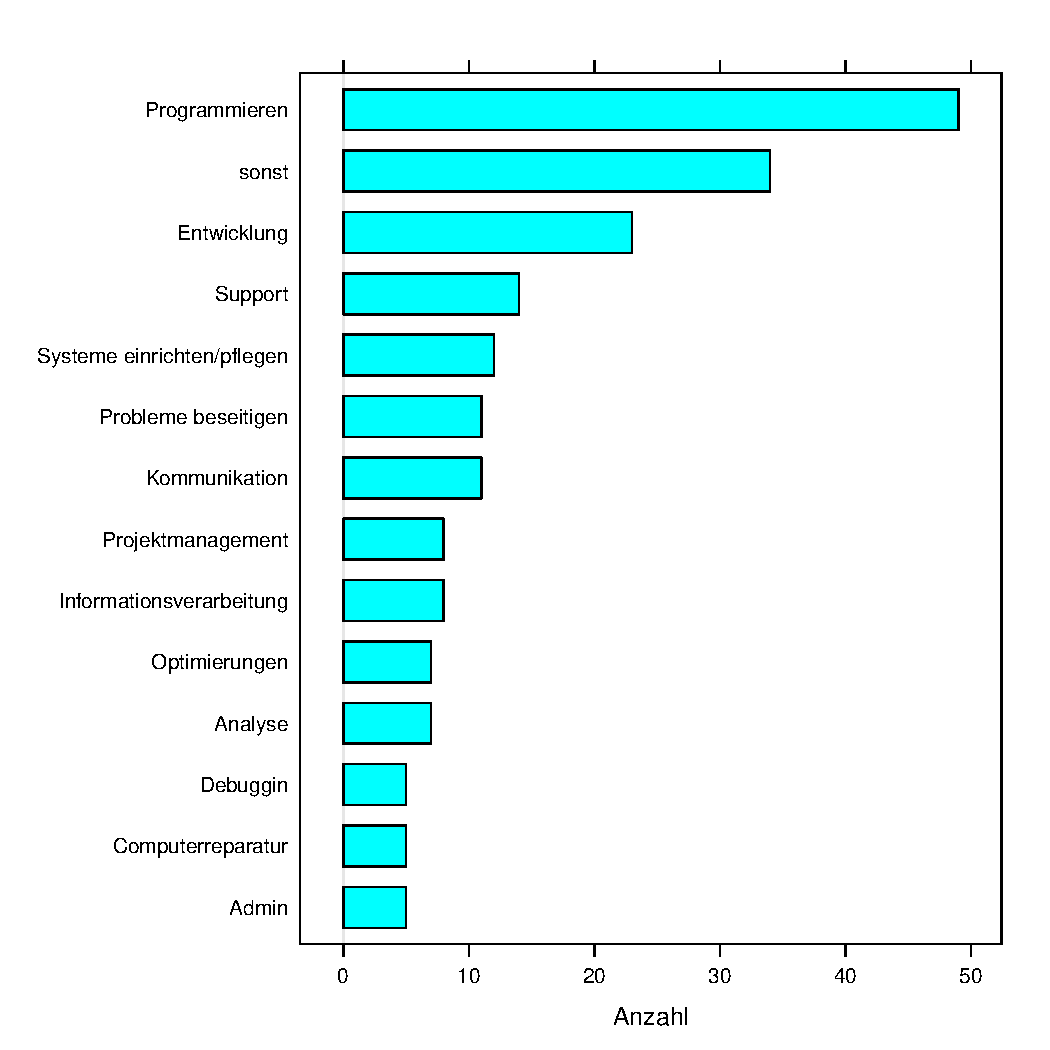
\includegraphics[width=\linewidth]{figure/chart_jobs-1} 

\end{knitrout}
    \caption{Aufgaben von InformatikerInnen nach Bekanntheitsgrad der ProbandInnen mit diesen}
    \label{fig:jobs}
\end{figure}

Bez\"uglich des Alters konnten einige Unterschiede in den Antworten der ProbandInnen festgestellt werden. So sch\"atzen ProbandInnen der \"alteren Generation von \"uber 40 die mit Computerspielen verbrachte Zeit von Informatikern deutlich geringer ein, wie in Abbildung \ref{fig:games_alter} zu sehen. Im linken Graphen der \"alteren ProbandInnen liegt der Modus der Antworten bei \emph{gelegentlichem} Computerspielen, also seltener als w\"ochentlich. Im Gegensatz dazu antworten bei den j\"ungeren ProbandInnen zwei Drittel mit einer gesch\"atzten H\"aufigkeit von mehreren Stunden Computerspiele in der Woche.  

\begin{figure}
\begin{knitrout}
\definecolor{shadecolor}{rgb}{0.969, 0.969, 0.969}\color{fgcolor}
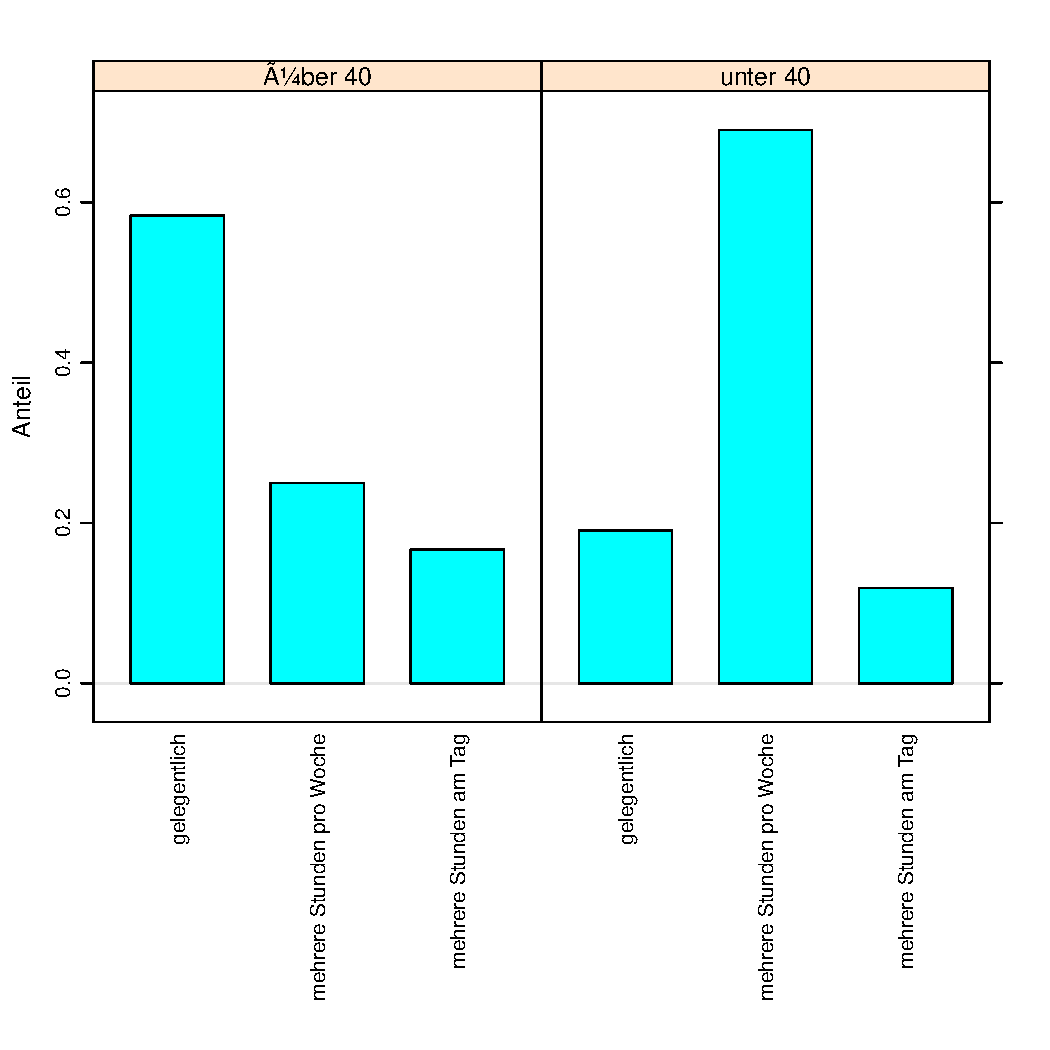
\includegraphics[width=\linewidth]{figure/chart_age-games-1} 

\end{knitrout}
    \caption{Gesch\"atzte mit Computerspielen verbrachte Zeit in Abh\"angigkeit vom Alter der ProbandInnen}
    \label{fig:games_alter}
\end{figure}

Unterschiede finden sich auch darin, wie die ProbandInnen den Beziehungsstand von InformatikerInnen einschätzen. Eine Gegen\"uberstellung ist in Abbildung \ref{fig:beziehung_alter} zu sehen. ProbandInnen des \"alteren Semesters vermuten eher, dass sich die meisten InformatikerInnen in einer Beziehung oder sogar in einer langj\"ahrigen Beziehung befinden. Von den unter 40-j\"ahrigen sch\"atzen etwa zwei F\"unftel der ProbandInnen die meisten InformatikerInnen als ledig ein.

\begin{figure}
\begin{knitrout}
\definecolor{shadecolor}{rgb}{0.969, 0.969, 0.969}\color{fgcolor}
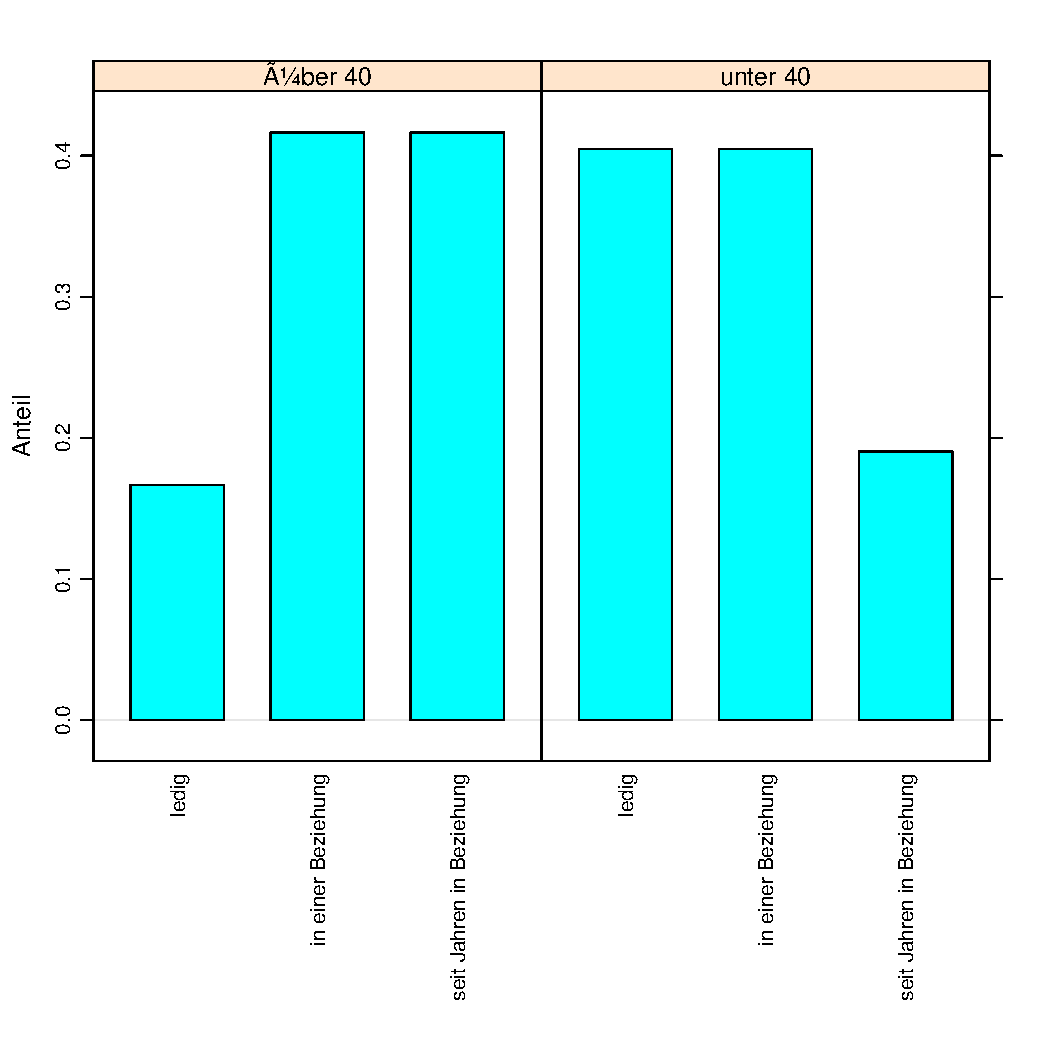
\includegraphics[width=\linewidth]{figure/chart_age-beziehung-1} 

\end{knitrout}
    \caption{Gesch\"atzter Beziehungsstand in Abh\"angigkeit vom Alter der ProbandInnen}
    \label{fig:beziehung_alter}
\end{figure}

Anhand der von uns erhobenen Daten kann nicht eingesch\"atzt werden, in wie weit diese generationsspezifischen Unterschiede in der Wahrnehmung von InformatikerInnen sich auf eben diese beschr\"anken, oder allgemein f\"ur die Wahrnehmung der gesamten Bev\"olkerung stehen.

F\"ur die Unterschiede k\"onnten zudem verschiedene Wertvorstellungen unbewusst verantwortlich sein. So wird beispielsweise die Familienplanung heutzutage h\"aufig hinter die Karriere zur\"uckgestellt. Zudem ist das Computerspielen inzwischen auch bei nicht InformatikerInnen weit verbreitet, die dann ebenfalls mehr Zeit damit verbringen.

Ein weiterer interessanter Punkt in unserer Analyse ist die gesch\"atzte Frauenquote bei den InformatikerInnen (vgl. Abbildung \ref{fig:frauenquote}). Kein einzige Proband hat den Anteil der Frauen in der Informatik h\"oher als 40 \% eingesch\"atzt. Die breite Streuung liegt vermutlich stark an den jeweiligen pers\"onlichen Erfahrungen. Zum Vergleich waren an der FU Berlin im Wintersemester 16/17 im Bachelorstudium etwa 20 \% und im Masterstudium rund 10 \% Frauen im Studium Informatik eingeschrieben.  Auffallend an dieser Analyse ist die sehr geringe Streuung bei Probanden mit nur beruflichem Kontakt zu Informatikern. Zwar nimmt der Anteil weiblicher Studierender in der Informatik in letzter Zeit stark zu, jedoch sind diese wohl zum Gro{\ss}teil entweder noch nicht im Berufsleben angekommen, oder sie arbeiten aufgrund des h\"oheren Abschlusses eher an Projekten und weniger im Supportbereich, der ja doch am meisten Kontakt mit anderen Mitarbeitern bietet.

\begin{figure}
\begin{knitrout}
\definecolor{shadecolor}{rgb}{0.969, 0.969, 0.969}\color{fgcolor}
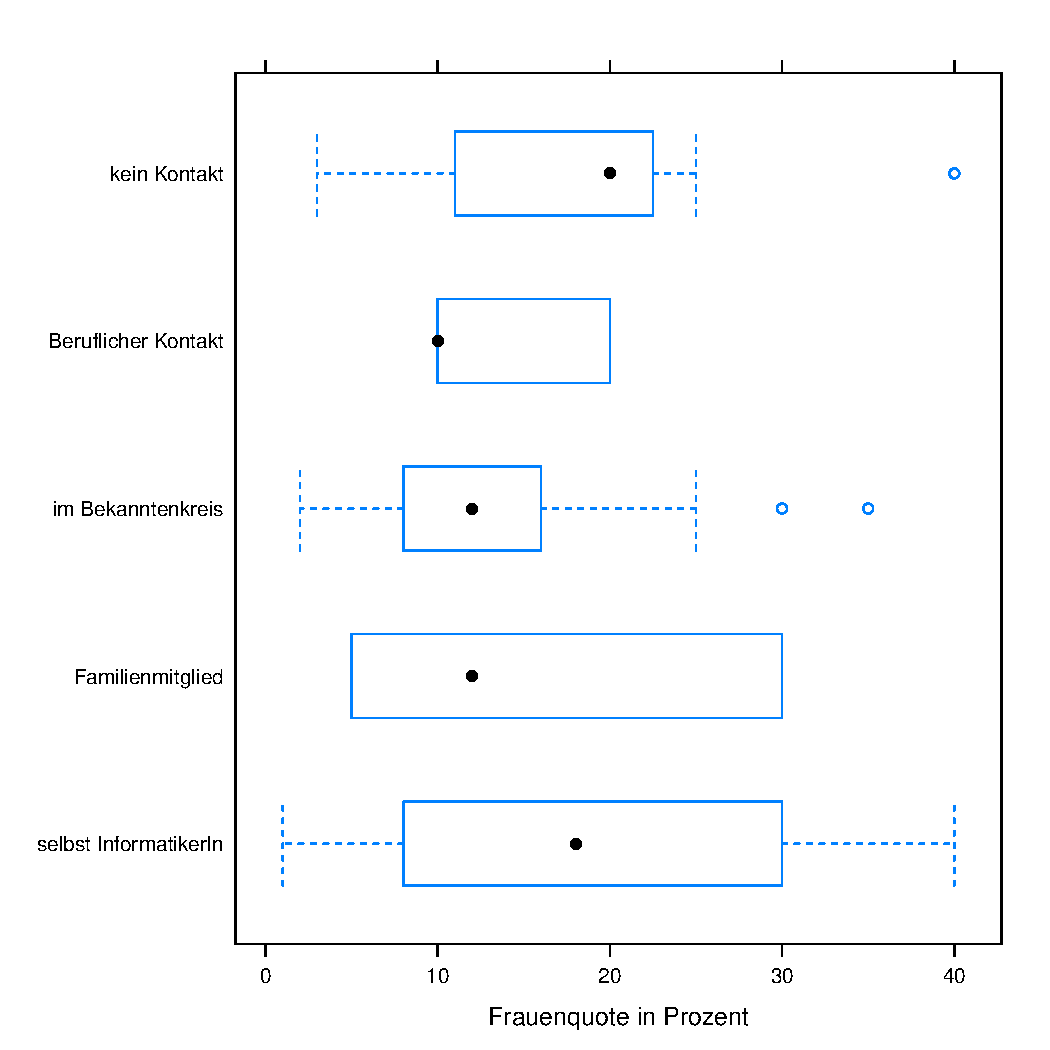
\includegraphics[width=\linewidth]{figure/chart_quote-1} 

\end{knitrout}
    \caption{Gesch\"atzter Frauenquote in Abh\"angigkeit vom Kontakt mit InformatikerInnen}
    \label{fig:frauenquote}
\end{figure}

\section[]{Schlussfolgerungen}
Summary of the most important insights from the analysis and
answer to the research question with respect to your hypotheses.
If answering your research question is not possible, discuss why.
Discussion of the threats to validity and the survey's
shortcomings as well as evaluation of credibility and relevance.


\section[]{Reflektion}

What did you learn from (or became aware of during) this project with
respect to: choice and formulation of a research question,
drafting and implementation of a questionnaire,
recruitment of participants,
data collection, evaluation, and drawing of conclusions?
Evaluate your approach in view of the general approach for
empiricism (see
\url{http://www.inf.fu-berlin.de/inst/ag-se/teaching/V-EMPIR-2017/11_generic_method.pdf}).


% For printing all bib entries; remove to only print actually cited entries
\nocite{*}

\bibliography{sample}


\appendix

\section{Anschreiben}

Liebe StudentInnen,\\
im Rahmen des Kurses “Empirische Bewertung in der Informatik” an der Freien Universität Berlin führen wir eine Studie zum Thema “Wahrnehmung der InformatikerInnen in der Gesellschaft” durch. Mit dieser Umfrage wollen wir herausfinden, ob es zwischen verschiedenen Generationen eine unterschiedliche Wahrnehmung gegenüber Informatikern gibt. Wir suchen dafür interessierte Teilnehmer und Teilnehmerinnen. Der zeitliche Aufwand beträgt maximal 10 Minuten.\\
Die Umfrage ist selbstverständlich anonym. Der Umfragezeitraum endet am 29.06.2017.\\

Die Umfrage finden ihr  unter https://goo.gl/forms/FRzYsoV646aLGHBc2 \\

Wenn ihr an den Ergebnissen der Umfrage interessiert seid, schreiben uns eine E-Mail an jana.kirschner@fu-berlin.de und wir senden euch die Ergebnisse, sobald sie uns vorliegen.\\ \\

Mit freundlichen Grüßen\\
und vielen Dank für eure Teilnahme\\ 
das Team der Freien Universität Berlin\\



\section{Fragebogen}

...


\section{Rohdaten und Auswertungskripte}

URL zum Download der Rohdaten und der R-Analyseskripte, die sich direkt auf den
Rohdaten ausführen lassen.
Idealerweise ein Git-Repository.

\end{document}
